\section{Integrasi \emph{Plugin} Untuk Simulasi}
\label{sec:integrasiplugin}

Agar sistem yang ada di simulasi dapat bekerja dan terabstraksi selayaknya sistem yang ada pada \emph{real robot},
  model yang ada di simulasi perlu diintegrasikan dengan \emph{plugin} yang memungkinkan sensor dan aktuator yang ada di simulasi berkomunikasi dengan \emph{node} lain menggunakan sistem komunikasi antar-proses ROS 2.
  Agar dapat bekerja dengan model yang telah dibuat, \emph{plugin} tersebut nantinya perlu disematkan pada \emph{file} SDFormat dari model robot sebagai \emph{child element} dalam bentuk \emph{plugin element}.

\begin{figure} [ht]
  \centering
  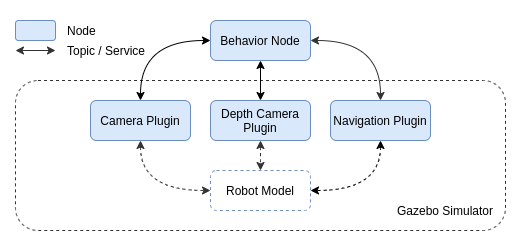
\includegraphics[scale=0.5]{gambar/integrasi-plugin-simulasi.png}
  \caption{Diagram integrasi \emph{plugin} untuk simulasi.}
  \label{fig:integrasipluginsimulasi}
\end{figure}

Seperti yang terlihat pada gambar \ref{fig:integrasipluginsimulasi},
  model robot akan diintegrasikan dengan tiga buah \emph{plugin},
  \emph{camera plugin} yang akan terabstraksi sebagai komponen kamera,
  \emph{depth camera plugin} yang akan terabstraksi sebagai komponen \emph{depth camera},
  dan \emph{navigation plugin} yang akan terabstraksi sebagai komponen navigasi.
Ketiga plugin tersebut nantinya akan dibentuk sebagai \emph{ROS 2 node} sehingga memungkinkan komunikasi dengan \emph{node} lain,
  termasuk \emph{behavior node} yang akan mengatur tingkah laku dari robot selama pengujian.

\subimport{4-integrasi-plugin}{1-navigation-plugin.tex}
\subimport{4-integrasi-plugin}{2-camera-plugin.tex}
\subimport{4-integrasi-plugin}{3-depth-camera-plugin.tex}
\subimport{4-integrasi-plugin}{4-legs-plugin.tex}
